
In this section, we study the externalities of exploration at a group
level, quantifying how much the presence of one population impacts the
rewards of another in an online learning system. We consider linear
contextual bandits in a setting in which there are two underlying user
populations, called the \emph{majority} and the \emph{minority}. The
user who arrives at round $t$ is assumed to come from the majority
population with some fixed probability and the minority population
otherwise, and the population from which the user comes is known to
the learner. The tuple of context vectors at time $t$ is then drawn
independently from a fixed group-specific distribution.

We assume there is a
single hidden vector $\theta$, and that the distribution of rewards conditioned
on the chosen context vector is
the same for both groups. Only the distribution over tuples of
available context vectors differs between groups. This implies that
externalities cannot be explained by the absence of a good policy,
since there always exists a policy that is simultaneously optimal for
everyone. This allows us to focus only on externalities inherent to the
process of exploration.

We define the \emph{minority regret} to be the regret experienced by
the minority. The \emph{group
  externality} imposed on the minority by the majority is then the
difference between the minority regret of an algorithm run on the
minority alone and the minority regret of the same algorithm run on
the full population. A negative group externality implies that the
minority is worse off due to the presence of the majority.
It is generally more meaningful to bound the multiplicative
difference between the minority regret obtained with and without the
majority present. Several of our results have this form. \looseness=-1

We first ask whether large group externalities can exist. We show that
on a simple toy example, a large negative group externality arises
under LinUCB, while a slight variant of this example leads to a large
positive externality. Put another way, more available data can lead to
either better or worse outcomes for the users of a system. We show
that this general phenomenon is unavoidable. That is, no algorithm can
simultaneously approximate the minority regret of LinUCB run on the
full population and LinUCB run on the minority alone, up to any
$o(\sqrt{T})$ multiplicative factor.

\subsection{Two-Bridge Instance}
We consider a toy example, motivated by a scenario in which a learner
is choosing driving routes for two groups of users. Each user starts
at point $A$, $B$, or $C$, and wants to get to the same destination,
point $D$, which requires taking one of two bridges, as shown in
Figure~\ref{fig:bridges}. The travel costs for each of the two bridges
are unknown. For simplicity, assume all other edges are known to have
0 cost.

Suppose that 95\% of users are in the majority group. All of these
users start at point $A$ and have access only to the top bridge. The
other 5\% are in the minority. Of these users, 95\% start at point
$C$, from which they have access only to the bottom bridge. The
remaining 5\% of the minority users start at point $B$, and have
access to both bridges.

\begin{figure}
\centering
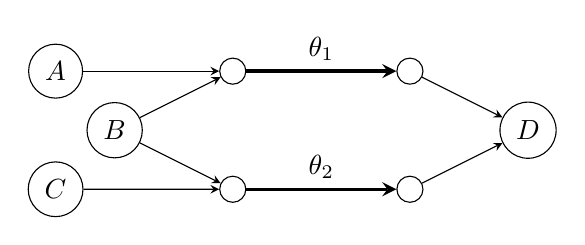
\begin{tikzpicture}[scale=.75]
\node[circle, draw] (A) at (-2,-1) {$A$};
\node[circle, draw] (B) at (-1,-2) {$B$};
\node[circle, draw] (C) at (-2,-3) {$C$};
\node[circle, draw] (s1) at (1,-1) {};
\node[circle, draw] (s2) at (1,-3) {};
\node[circle, draw] (e1) at (4,-1) {};
\node[circle, draw] (e2) at (4,-3) {};
\node[circle, draw] (D) at (6,-2) {$D$};
\draw[->,draw,>=stealth] (A) -- (s1);
\draw[->,draw,>=stealth] (B) -- (s1);
\draw[->,draw,>=stealth] (B) -- (s2);
\draw[->,draw,>=stealth] (C) -- (s2);
\draw[->,draw,>=stealth,very thick] (s1) -- (e1) node[midway,above] {$\theta_1$};
\draw[->,draw,>=stealth,very thick] (s2) -- (e2) node[midway,above] {$\theta_2$};
\draw[->,draw,>=stealth] (e1) -- (D);
\draw[->,draw,>=stealth] (e2) -- (D);
\end{tikzpicture}
\caption{Visual illustration of the two-bridge instance. \label{fig:bridges}}
\end{figure}

Consider the behavior of an algorithm that follows the principle of
optimism under uncertainty.  If run on the full user population, it
will quickly collect many observations of the commute time for the top
bridge since all users in the majority group must travel over the top
bridge.  It will collect relatively fewer observations of the commute
time over the bottom bridge.  Therefore, when the algorithm is faced
with a member of the minority population who starts at point $B$, the
algorithm will likely send this user over the bottom bridge in order
to collect more data and improve its estimate. \looseness=-1

If the same algorithm is instead run on the minority alone, it will
quickly collect many more observations of the commute time for the
bottom bridge relative to the top.
Now when the algorithm is faced with a user who starts
at point $B$, it will likely send her over the top bridge.

Which is better depends on which bridge has the longer commute time.
If the top bridge is the better option, then the presence of the
majority imposes a negative externality on the minority. If not, then
the presence of the majority helps. These two scenarios may be
difficult to distinguish.

This toy example can be formalized in the linear contextual bandits
framework. There are two underlying actions (the two bridges), but
these actions are not always available. To capture this, we define a
parameter vector $\theta$ in $[0, 1]^2$, with the two coordinates
$\theta_1$ and $\theta_2$ representing the expected rewards for taking
the top and bottom bridge respectively. (Though we motivated
the example in terms of costs, it can be expressed equivalently in
terms of rewards.) There are two possible context vectors:
$[1 ~ 0]\tran$ and $[0 ~ 1]\tran$. A user has available an action with
context vector $[1 ~ 0]\tran$ if and only if she has access to the top
bridge. Similarly, she has available an action with context vector
$[0 ~ 1]\tran$ if and only if she has access to the bottom bridge. The
instance can then be formalized as follows.



\begin{definition}[Two-Bridge Instance]
  The \emph{two-bridge instance} is an instance of linear contextual
  bandits. On each round $t$, the user who arrives is from the
  majority population with probability 0.95, in which case
  $x_{1, t} = x_{2, t} = [1 ~ 0]\tran$. Otherwise, the user is in the
  minority. In this case, with probability 0.95,
  $x_{1,t} = x_{2,t} = [0 ~ 1]\tran$ (based on
  Figure~\ref{fig:bridges}, we call these $C$ rounds), while with probability 0.05, $x_{1,t} = [1 ~ 0]\tran$ and
  $x_{2,t} = [0 ~ 1]\tran$ ($B$ rounds). We consider two
  values for the hidden parameter vector $\theta$,
  $\thetazero = [1/2 \ ~ 1/2 - \varepsilon]\tran$ and
  $\thetaone = [1/2 - \varepsilon \ ~ 1/2]\tran$ where
  $\varepsilon = 1/\sqrt{T}$.
\end{definition}


\subsection{Performance of LinUCB}


We start by analyzing the performance of LinUCB on the two-bridge
instance.  Our main result formalizes the intuition above, showing
that when $\theta = \thetazero$ (that is, the top bridge is better)
the majority imposes a large negative group externality on the
minority, while the majority imposes a large positive externality when
$\theta = \thetaone$. We assume rewards are $1$-subgaussian.%
\footnote{A random variable $X$ is called $\sigma$-subgaussian if $E[e^{\sigma X^2}]<\infty$. A special case is Gaussians with variance $\sigma^2$.}


\begin{theorem}
  Consider LinUCB with any interval width function $f$ satisfying
  $f(t) \ge 2\sqrt{\log(T)}$.%
  \footnote{For instance, the interval width function in Equation~\eqref{eq:Abbasi-f} satisfies this condition whenever $d c_0\geq 4$, so one can either set $c_0\geq 2$, or add two more dimensions to the problem instance (and set $\theta_3 = \theta_4 =0$).}
   On the two-bridge instance,
  assuming $1$-subgaussian noise on the rewards, when
  $\theta = \thetazero$, LinUCB achieves expected minority regret
  $O(1)$
  when run on the minority alone, but $\Omega(\sqrt{T})$ when run on
  the full population.  In contrast, when $\theta = \thetaone$, LinUCB
  achieves expected minority regret $O(1)$ when run on the full
  population, but $\Omega(\sqrt{T})$ when run on the minority alone.
\label{thm:twobridgelinucb}
\end{theorem}

We omit the proofs of the $\Omega(\sqrt{T})$ lower bounds, which both
follow a similar structure to the one used in the proof of the general
impossibility result in Section~\ref{sec:impossibility}; in fact, both
of these lower bounds could be stated as an immediate corollary of
Theorem~\ref{thm:indistinguishability}.  Essentially, an argument
based on KL-divergence shows that it is difficult to distinguish
between the case in which $\theta = \thetazero$ and the case in which
$\theta = \thetaone$, and therefore LinUCB must choose similar actions
in these two cases.

To prove the $O(1)$ upper bounds, we make heavy use of the special
structure of the two-bridge instance, which significantly simplifies
the analysis of LinUCB. We exploit the fact that the only context
vectors available to the learner are the basis vectors $[1 ~ 0]\tran$
and $[0 ~ 1]\tran$, which essentially makes this an instance of
sleeping bandits~\citep{SleepingBandits-ml10}. In this special case,
the covariance matrix $Z_t$ is always diagonal, which simplifies
Equation~\eqref{eq:linucb_def} and leads to LinUCB choosing the $i$th
basis, where $i$ maximizes $(\thetahatt)_i + f(t)/\sqrt{(Z_t)_{ii}}$ and
$(Z_t)_{ii}$ is simply the number of times that this basis vector was
already chosen. Additionally, in this setting $(\thetahatt)_i$ is just the
average reward observed for the $i$th basis vector, allowing us to
bound the difference between each $(\thetahatt)_i$ and $\theta_i$ using
standard concentration techniques. Using this, we show that with high
probability, after a logarithmic number of rounds---during which the
learner can amass at most $O(1)$ regret since the worst-case regret on
any round is $\varepsilon = 1/\sqrt{T}$---the probability that LinUCB
chooses the wrong action on a $B$ round is small ($O(1/\sqrt{T})$).
This leads to constant regret on expectation.



\subsection{An Impossibility Result}
\label{sec:impossibility}

It is natural to ask whether it is possible to design an algorithm
that can distinguish between the two scenarios analyzed above,
obtaining minority regret that is close to the best of LinUCB run on
the minority alone and LinUCB run on the full population on any
problem instance. In this section, we show that the answer is no. In
particular, we prove that on the two-bridge instance, if
$\Pr[\theta = \thetazero] = \Pr[\theta = \thetaone] = 1/2$, then any
algorithm must suffer $\Omega(\sqrt{T})$ regret on expectation (and
therefore $\Omega(\sqrt{T})$ minority regret, since all regret is
incurred by minority users).

To prove this result, we begin by formalizing the idea that it is hard
to distinguish between the case in which $\theta = \thetazero$ and the
case in which $\theta = \thetaone$. To do so, we bound the
KL-divergence between the joint distributions over the sequences of
context vectors, actions taken by the given algorithm, and the given
algorithm's rewards that are induced by the two choices of $\theta$.
By applying the high-probability Pinsker lemma~\citep{T09}, we show
that a low KL-divergence between these distributions implies that the
algorithm must be likely either to choose the top bridge on $B$ rounds
more than half the time when the bottom bridge is better or to choose the
bottom bridge on $B$ rounds more than half the time when the top
bridge is better, either of which would lead to high
($\Omega(\sqrt{T})$) regret as long as the number of $B$ rounds is
sufficiently large. To finish the proof, we use a simple Chernoff
bound to show that the number of $B$ rounds is large with high
probability.

To derive the KL-divergence bound, we make use of the assumption that
the realized rewards $r_t$ at each round are either $0$ or $1$.  This
assumption is not strictly necessary.  An analogous argument could be
made, for instance, for real-valued rewards with Gaussian noise.

\begin{theorem} \label{thm:indistinguishability}
On the two-bridge instance with realized rewards $r_t \in \{0,1\}$, any algorithm must incur $\Omega(\sqrt{T})$ minority regret
in expectation when $\Pr[\theta = \thetazero] = \Pr[\theta = \thetaone] = \tfrac12$.
\end{theorem}

Note that ``any algorithm'' here includes algorithms run on the
minority alone, essentially ignoring data from the majority.
Theorems~\ref{thm:twobridgelinucb} and~\ref{thm:indistinguishability}
immediately imply the following corollary.

\begin{corollary}
No algorithm can simultaneously approximate the minority regret of both LinUCB run on the minority and LinUCB run on the full population up to any $o(\sqrt{T})$ multiplicative factor.
\end{corollary}
